
\chapter{Service Cutter Design \& Implementation}
\label{cha:implementation}

To satisfy the requirements defined in Section \ref{cha:requirements}, the Service Cutter was built. This chapter documents design and implementation aspects.


\section{Service Cutter Process}
%TODO weglassen?

The Service Cutter's decomposition calculation is based on nanoentities. In a first step, nanoentities are inserted into the Service Cutter and define a system to be analyzed. The user then defines meta data on the nanoentities and their relations in a second step. During the third step, the user runs the decomposition process to receive suggestions of how the nanoentities could be split into services. He finally analyzes these candidate service cuts and compares it with his own expectations. 

%TODO add process chart. e.g. steps: |1> >2> >3> >4> or bpmn?

\subsection{Step 1: Model Initialization}

In this step a model representing a system to be analyzed is created in the Service Cutter. The user defines all nanoentities relevant for his domain. 

Importing these nanoentities is possible either as a list of nanoentities or parsed from an \gls{ERM} defined in a self defined JSON representation.

%ZIO: a bit too short
%TODO add REST URI and json example

\subsection{Step 2: Model Description}

In the second step the model is described with meta data that is used by the Service Cutter to calculate coupling between nanoentities for each coupling criteria. This meta data is imported using user representations in a self defined JSON representation.

%TODO document REST URIs and JSON formats 	

Almost all nanoentities are related in some way to other nanoentities. The concept of a coupling criterion described in Chapter \ref{cha:decomposition} is used to characterize such relations. In this step the user needs to enhance the model with meta information about the nanoentities's characteristics and relations to each other. To improve usability well known concepts like use cases are defined as user representation which can be used to enhance the model. 

Importing the user representation should either be done over a RESTful HTTP API in a self defined JSON format or using a wizard within the Service Cutter's \gls{UI}.

\subsection{Step 3: Decomposition}

Once the user has added all nanoentities and coupling criteria he can start the decomposition process. An algorithm groups nanoentities in a way that a good decomposition solution as described in Section \ref{sec:decompositionRequirements} is found. 

The algorithm will then present the candidate service cuts to the user.

\subsection{Step 4: Working with Candidate Service Cuts}

Once candidate service cuts have been presented, the user needs to interpret them and compare it with his own expectations. There are multiple ways the provided data could be further used in the process of a software engineering project.

The candidate service cuts can be exported as a \gls{JSON} file for further processing.

\lstset{
   	language=JavaScript,
   	tabsize=3,
   	%frame=lines,
   	caption=JSON export of a candidate service cut,
   	label=code:cut-bookingsample,
   	frame=shadowbox,
   	rulesepcolor=\color{gray},
   	xleftmargin=20pt,
   	framexleftmargin=15pt,
   	keywordstyle=\color{blue}\bf,
   	commentstyle=\color{OliveGreen},
   	stringstyle=\color{red},
   	numbers=left,
   	numberstyle=\tiny,
   	numbersep=5pt,
   	breaklines=true,
   	showstringspaces=false,
   	basicstyle=\footnotesize}
\lstinputlisting{code/CandidateServiceCut-BookingSample.json}


\section{Service Decomposition using a Weighted Undirected Graph}
\label{subsec:approach1_graph}

Service decomposition describes the task of grouping nanoentities into services. Achieving a good solution according to the defined coupling criteria as described in Section \ref{sec:decompositionRequirements} requires a non trivial algorithm. We approach this problem by using a weighted undirected graph and clustering algorithms as described in this section. Other approaches have been evaluated but could not provide satisfying results as documented in Appendix \ref{appendix:decompositionAppraoches}.

\begin{minipage}[t]{0.6\textwidth}
	\setlength{\parskip}{5pt plus 0.1pt}	
	To create a weighted undirected graph, every nanoentity in the model is represented by a node. Edges define a relationship between two nanoentities. The weight on each edge shows how \textit{close} or \textit{cohesive} two nanoentities are. The higher the weight, the more likely they should belong to the same service. Figure \ref{fig:weighted_graph} shows an abstract example of such a graph.
\end{minipage}
\begin{minipage}[t]{0.4\textwidth}
	
	
	\begin{figure}[H]
		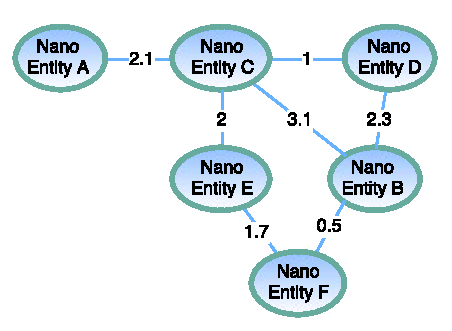
\includegraphics[scale=0.8]{diagrams/weighted_graph.pdf}
		\caption{Example of a Weighted Graph}
		\label{fig:weighted_graph}
	\end{figure}
	
\end{minipage}

\begin{minipage}[t]{0.5\textwidth}
	\setlength{\parskip}{5pt plus 0.1pt}
	
	%ZIO: a bit abstract. concrete example needed to appreciate. input/output jedes schrittes nennen/zeigen
	
	Figure \ref{fig:graph_approach} outlines a solution sketch for this approach. User representations like an \gls{ERM} or use cases are imported. The \textit{importer} component extracts the nanoentities and the coupling meta data stores this information in a database.
	
	The \textit{Solver} then creates all vertices from the nanoentities and builds weighted edges between them according to the stored coupling criteria instances. This task is complex for the following reasons:
	
	\begin{enumerate}
		\item Coupling criteria are not homogeneous as described in Section \ref{subsec:couplingCriteriaOverview}. Cohesiveness criteria describe why nanoentities should belong to the same service while compatibility criteria ask for separation of nanoentities. Constraints criteria might require both. Criteria of type communication need to be processed differently as they define which nanoentities are suitable to be transmitted across services. The information from all types needs to be represented with a single unit to define a number used as a weight of an edge.
		
		\item Using a single number with only one unit of measurement bears the risk of unintended change of the relative importance between the coupling criteria. It is important to carefully assure that each coupling criteria uses the same range of numbers to allow comparison and prioritization of each criteria.   
		
		\item To allow the user to define the specific requirements of his system, priorities per coupling criteria can optionally be defined to influence the weights of each coupling criteria instance.
	\end{enumerate}
	
	The \textit{Clustering Algorithm} then analyzes the graph and creates clusters of nanoentities so that as few edges as possible need to be cut.	
	
\end{minipage}
\begin{minipage}[t]{0.5\textwidth}
	\begin{figure}[H]
		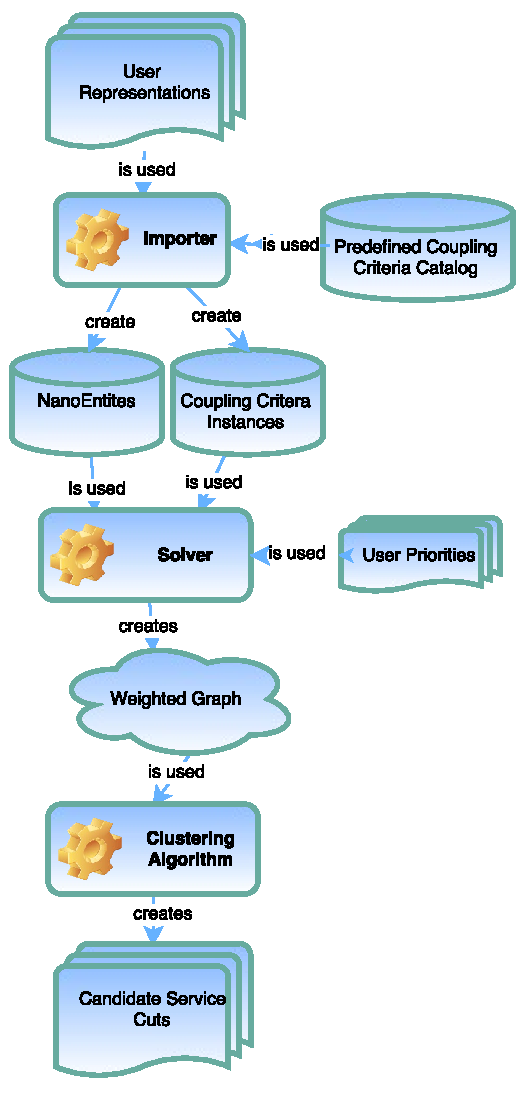
\includegraphics[scale=1.0]{diagrams/graph_approach.pdf}
		\caption{Solution Sketch for a Weighted Graph with a Clustering Algorithm}
		\label{fig:graph_approach}
	\end{figure}
\end{minipage}

\subsection{Performance}

%TODO: performance of algorithm against graph building performance?
%TODO: compare performance of algorithms?
%TODO: weglassen? nach hinten verschieben?

The theoretical number of nodes may cause performance problems. The maximum number of edges in a graph can be described using a formula: A graph of $n$ nodes, where every node is connected to all other nodes, has $e$ edges.

\begin{displaymath}
e = \frac{n(n-1)}{2}
\end{displaymath}

The number of edges grows almost quadratically as shown in Table \ref{tab:edgesCount}.

\begin{table}[H]
	\centering
	\caption{Maximum number of edges in an undirected graph}
	\label{tab:edgesCount}
	\begin{tabular}{|r|r|}
		\hline \textbf{Nodes} $n$ & \textbf{Edges} $e$ \\ 
		\hline 2 & 1 \\ 
		\hline 3 & 3 \\ 
		\hline 20 & 190 \\ 
		\hline 50 & 1'225 \\ 
		\hline 100 & 4'950 \\ 
		\hline 2000 & 1'999'999 \\ 
		\hline 
	\end{tabular} 
\end{table}

Our implementation however will unlikely have anything close to the theoretical number of edges as:
\begin{itemize}
	\item Coupling of type \textit{Cohesiveness} only adds edges where nanoservices are in a relationship with each other.
	\item Coupling of type \textit{Compatibility} only adds a negative score (penalty) to existing relationships.
	\item Coupling of type \textit{Constraint} only removes existing edges.
	%todo communication
\end{itemize}

The number of edges can therefore only cause problems when a Cohesiveness coupling is specified that includes a large number of nodes. An example of such a coupling is for a use case including a very large number of nanoentities which is a very unlikely case. We therefore conclude that the number of edges is probably not an issue.


\section{Clustering Algorithms}

A clustering algorithm is required to split the undirected, weighted graph into groups of nodes having as few connections between the clusters as possible. 

A full comparison of the evaluated algorithms is attached in Appendix \ref{appendix:graphClusteringAlgs}.

The remaining three algorithm candidates are Girvan-Newman, MCL, and Leung. Leung is provided by the GraphStream project. Girvan-Newman and MCL are implemented as Gephi plugins. Gephi is a desktop platform with a well developed \gls{UI} to explore and visualize complex graphs and network systems. The platform provides a toolkit to use its functionality without a \gls{UI}.  The source code of the algorithms can be extracted from the plugins as \gls{JAR} files using the UnpackNBM tool\cite{unpackNBM}.

Table \ref{tab:clusterAlgorithms} documents the detailed evaluation of the three candidate algorithms. 

\begin{table}[H]
	\centering
	\caption{Evaluation of cluster algorithms}
	\label{tab:clusterAlgorithms}
	\begin{tabular}{|p{2.2cm}|p{4cm}|p{4cm}|p{4cm}|}
		\hline
		& \textbf{MCL}               & \textbf{Leung}                    & \textbf{Girvan-Newman}  \\ \hline
		Author              & Stijn van Dongen\cite{markovCluster} & U. N. Raghavan\cite{raghavan}, Ian X.Y. Leung\cite{leung}    & M. E. J. Newman, M. Girvan\cite{girvan} \\ \hline
		Year                & 2000                       & 2007/2009                         & \multicolumn{1}{l|}{2003}                       \\ \hline
		Name                & Markov Cluster Algorithm   & Epidemic Label Propagation        & \multicolumn{1}{l|}{Girvan–Newman}              \\ \hline
		Approach            & Random walks               & Labels spread to their neighbours & Edge betweenness, based on shortest-paths       \\ \hline
		Performance \newline \textit{N: Nodes} \newline \textit{E: Edges}         & $O (N k^2)$ \newline \textit{k: pruning constant} \cite[p.126]{markovCluster} & $O( E N )$ \cite[p.3]{leung}                         & $O ( N^3 )$\cite[p.14]{girvan}       \\ \hline
		Java Implementation & Plugin of Gephi\cite{gephiMarkov} & GraphStream project\cite{leungGraphstream} & Plugin of Gephi\cite{gephiMarkov} \\ \hline
		Test result         & Bugs                       & Good                              & \multicolumn{1}{l|}{Good}                       \\ \hline
		Deterministic & No & No & Yes \\
		\hline
		Number of clusters parameter & No & No & Yes \\
		\hline
	\end{tabular}
\end{table}

The \gls{MCL} algorithm is theoretically suitable to calculate the clusters. However we found the Java implementation not to be mature enough as the output contains overlapping or missing nodes so that the \textit{distinct clusters} requirement is not met. Leung and Girvan-Newman are used in the Service Cutter and both provide good results as documented in Appendix \ref{appendix:serviceCutterAssessment}.

\subsection{Girvan-Newman}
\label{subsec:girvanNewman}
	

M. E. J. Newman and M. Girvan\cite{girvan} proposed to use a divisive approach to graph clustering. This approach repeatedly finds the least similar connected pair of vertices and removes the edges between them. The least similar connected pair is defined by \textit{edge betweennees} which can be calculated using different approaches as described by Girvan-Newman. The Gephi implementation used in the Service Cutter calculates edge betweenness as the number of shortest paths of any pair of vertices running through an edge. Edges with the highest edge betweenness are removed first. This process divides the graph into smaller and smaller components and can be stopped at any time to select the components at this time to be the graph clusters.

In the ordered graph in Figure \ref{fig:girvan-newman-process} Girvan-Newman would remove the edges in ascending order. The graph is split into 4 clusters after 2 iterations.

\begin{figure}[H]
	\begin{center}
		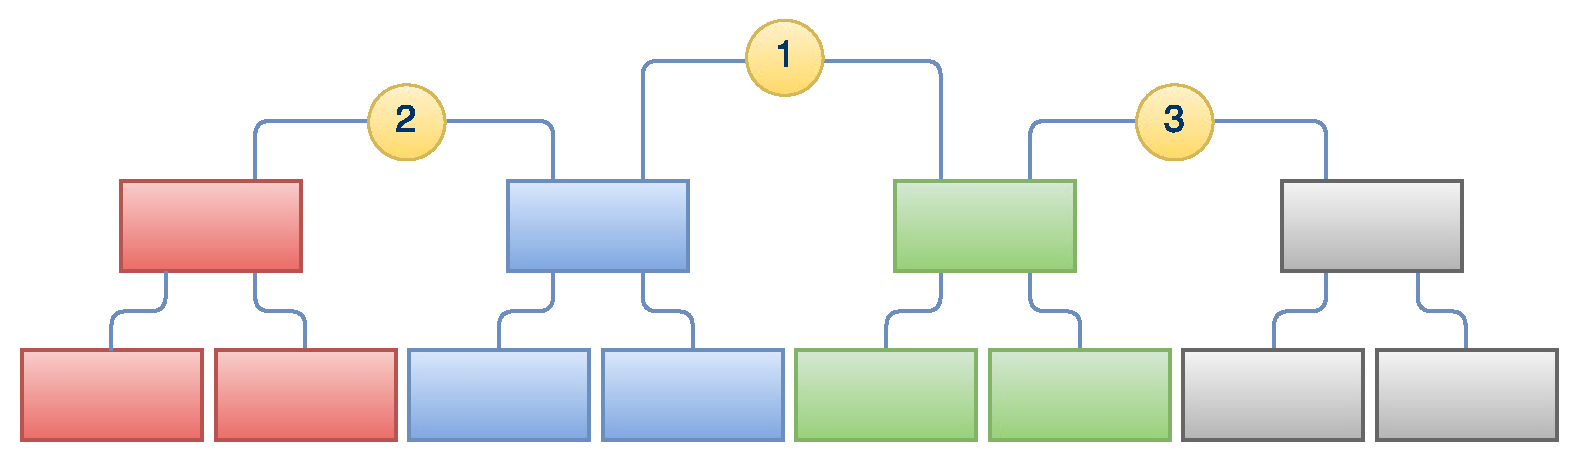
\includegraphics[scale=0.45]{diagrams/Girvan-Newman-Process.pdf}
	\end{center}
	\caption{Girvan-Newman forms clusters by removing edges iteratively}
	\label{fig:girvan-newman-process}
\end{figure}

Girvan-Newman receives the number of clusters as a parameter and stops as soon as the desired number has been reached. One iteration might remove multiple edges with the maximum edge betweenness. One iteration can therefore produce numerous new clusters so that the requested number of clusters cannot be provided. In this case the gephi implementation looks for a result having the least difference in number of clusters. 

As this algorithm does not include random elements, the proposed clusters are always identical.

\subsection{Leung}
\label{sec:monsterclusters}

In 2009 Leung \textit{et al}\cite{leung} refined the \enquote{Epidemic Label Propagation} algorithm as proposed by Raghavan \textit{et al}\cite{raghavan} in 2007. 

Raghvan described the algorithm as follows: \enquote{Each node in the network chooses to
join the community to which the maximum number of its neighbors belong to, with ties broken uniformly randomly. We initialize every node with unique labels and let the labels propagate through the network. As the labels propagate, densely connected groups of nodes quickly reach a consensus on a unique label.}\cite[p. 4]{raghavan}.

Leung does not specify an order in which nodes are to be processed. Therefore the labels may spread differently in repeated runs. We witnessed varying clusters while testing the Service Cutter as document in Appendix \ref{appendix:serviceCutterAssessment}.

The algorithm occasionally forms so called \enquote{monster} families as described by Leung \textit{et al} resulting in a drop of cohesion in a cluster. 

\enquote{[\dots] certain communities do not form strong enough links to prevent a foreign \enquote{epidemic} to sweep through.}\cite[p. 5]{leung}

Leung \textit{et al} therefore refined the algorithm by adding a \enquote{Hop Attenuation Factor} $\delta$ to prevent labels from spreading across two clusters. He explains: \enquote{The value $\delta$ governs how far a particular label can spread as a function of the geodesic distance from its origin. This additional parameter adds in extra uncertainties
to the algorithm but may encourage a stronger local community to form before a large cluster start to dominate.}\cite[p. 5]{leung}

This parameters decelerates the propagation of a cluster from its origin and therefore encourages a stronger local cluster to form before a large cluster starts to dominate.

We observed monster clusters especially in the DDDSample documented in Appendix \ref{sec:dddSample} and were able to reduce their likelyhood by increasing the hop attenuation factor to a value of $\delta \approx 0.55$ compared to a default of $ \delta = 0.1$ as provided by the GraphStream implementation. We decided to keep the value of $\delta = 0.55$ as the default of the Service Cutter.

\subsection{Discussion}
\label{subsec:algoDiscussion}

Two main differences between Leung and Girvan-Newman algorithms are determinism and the number of clusters parameter. This section discusses the advantages and disadvantages of each.

\subsubsection{Determinism}

Results of a deterministic algorithm like Girvan-Newman can be reproduced by running the algorithm again with the same input data. The influence of different input data, scoring values and priorities can therefore be analyzed as the algorithm itself does not contain a random element.

A non-deterministic algorithm like Leung complicates analysis since changes in results cannot clearly be identified as consequence of changes in input or randomness. Furthermore results always need to be safely persisted and reloaded since they cannot be reliably reproduced. 

Nevertheless, the representative of our industry partner, W. Giersche, accurately pointed out that an element of randomness is not only a disadvantage. Running multiple algorithm cycles presents different solutions and outlines where the difficult architectural decisions reside.

\subsubsection{Number of Clusters Parameter}

Providing the number of clusters as a parameter to the algorithm has the advantage of analyzing the service decomposition with any possible number of services. This feature can be used to better understand the structure and coupling between parts of the analyzed system by running an analysis with a number of services that is not optimal. Requesting a high number of service provides indications of how services internally might be further decomposed into modules. 

Furthermore the parameter allows to help in the process of emerging from a monolithic architecture to service orientation as described in Section XXX.
%TODO ref

Nevertheless, algorithms requesting the number of services as a parameter hand over the responsibility to answer this critical question to the user instead of answering it itself. W. Giersche pointed out that architects are often prejudiced on the number of services their system should be composed of. Having the Service Cutter providing not only the content of each service but also the number of services challenges the user to reassess his ideas against the candidate service cuts provided. 

%TODO überleitung

\section{Scoring}

The scoring process rates the relation of two nanoentities with a score. A higher positive score states that these entities should be modeled in the same service while a negative score asks for a separation of the nanoentities into different services.

\begin{figure}[H]
	\begin{center}
		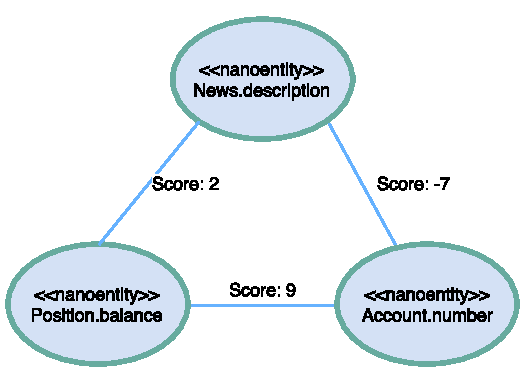
\includegraphics[scale=1]{diagrams/scoring_example.pdf}
		\caption{Simple Scoring Example}
		\label{fig:scoringExample}
	\end{center}
\end{figure}

Figure \ref{fig:scoringExample} shows three nanoentities from the Trading System (see Appendix \ref{sec:tradingSystem}) and their potential scores to each other. The relation \textit{Position.balance} to \textit{Account.number} has a high score as these nanoentities are often accessed in the same use cases and therefore get a high score from the \textit{Semantic Proximity} criterion. \textit{News.description} to \textit{Account.number} has a negative score. These nanoentities do not have common use cases and do not belong to the same entity, so the positive scores from \textit{cohesiveness} criteria are low or zero. Different characteristics like \textit{low} resilience requirements for \textit{News.description} and \textit{critical} resilience requirements for \textit{Account.number} lead to a negative score. 

In this simple example, the Service Cutter would most probably suggest two services, one with \textit{Account.number} and \textit{Position.balance} and another one with the \textit{News.description}.

\subsection{Single Dimensionality}
\label{subsec:singleDimensionality}

A big challenge with the graph based approach is that weights between nodes only have one dimension with a single unit of measurement. The edges can describe how close or cohesive two nanoentities are. This suites well to all coupling criteria of type cohesiveness as they describe reasons to combine nanoentities in the same service. Coupling criteria describing separation or incompatibility, where separation of nanoentities is asked by constraints or different nanoentity characteristics, cannot accurately be described using the weight on the edge.

Our approach to solve this problem is to introduce negative scores as shown in the example above. A negative score implies in the view of a coupling criterion that two fields should be separated into different services. If the negative score exceeds the positive score given by cohesiveness criteria, the edge between two nanoentity nodes is removed. 

This approach implies two disadvantages:

\begin{enumerate}
	\item By removing edges with a score lower than zero, information  about the need for separation is lost. The scores of $-120$ and $-1$ are processed equally. 
	\item Positive and negative scoring criteria must be balanced out. Too many negatively scoring criteria or high prioritization of such criteria leads to elimination of the positive data and therefore of all information available. 
\end{enumerate}


Nevertheless, the practical assessment documented in Appendix \ref{appendix:serviceCutterAssessment} proves effectiveness of this approach. Firstly, nanoentities without an edge are unlikely to be placed within the same service by the algorithm. Secondly, systems are described using an \gls{ERM} and use cases so that cohesiveness criteria are already provided with information. Negative scoring criteria only produce scores if nanoentities are described with characteristics not equal to the default characteristics. We furthermore defined the default priorities for each criteria, as described later in this section, in a way that positive scoring criteria are prioritized higher. 

%TODO: future work, find better solution and create a reference here

\subsection{Scoring Process}

To determine the final score between two nanoentities three steps are required. First every coupling criterion scores the relations it has information about. After that, priorities for each criterion are applied. Finally the prioritized scores of all criteria are summed up to a final score.

\subsubsection{Step 1: Score by Coupling Criterion}

Every coupling criterion calculates a score between $-10$ and $10$ for each nanoentity relation $AB$. 

\begin{displaymath}
criteria[i].score_{AB} = -10 ... 10
\end{displaymath}

A score of $10$ implies that \enquote{From the view of coupling criterion $i$, the nanoentities $A$ and $B$ should definitly reside in the same service.} A score of $-10$ implies that \enquote{From the view of coupling criterion $i$, the nanoentities $A$ and $B$ should definitly \textbf{not} reside in the same service.} 

The range from $-10$ to  $10$ was chosen to be able to compare scores of different coupling criterion with each other. A fixed range guarantees that not one criterion receives more importance than another one due to its scoring logic. Other ranges like $-1.00$ to $1.00$ would have worked as well, but in our opinion integer numbers are easier to understand for users than rational numbers. 

It is important to notice that not every criterion has to use the full possible range. Coupling criteria of type \textit{cohesiveness} tend to score only positive values, as they describe why nanoentities should be composed in the same service. Criteria of type \textit{compatibility} or \textit{constraints} on the other hand tend to score negative, as they describe reasons to split nanoentities into different services.

\subsubsection{Step 2: Prioritized Coupling Criteria}

In the second step, the coupling criteria are prioritized relatively to each other. Table \ref{tab:priorities} outlines all possible priorities.

\begin{table}[H]
	\centering
	\caption{Coupling Criterion Priorities}
	\label{tab:priorities}
	\begin{tabular}{|p{70pt}|p{30pt}|}
		\hline	
		Representation & Value  \\
		\hline
		IGNORE & 0  \\
		\hline
		XS & 0.5  \\
		\hline
		S & 1  \\
		\hline
		M & 3  \\
		\hline
		L & 5  \\
		\hline
		XL & 8  \\
		\hline
		XXL & 13  \\
		\hline
	\end{tabular}
\end{table}

The priorities are represented by t-shirt sizes each defining a priority value. By recommendation of W. Giersche, a representative of our industry partner, and inspired by agile estimation scales\footnote{Alex Yakyma wrote an insightful paper on why progressive estimations are efficient for teams\cite{estimation}.}, we chose a progressive and nearly exponential value sequence. 

Having very high values allows analyzing a system in the Service Cutter with focus on one or two coupling criteria only as giving a criterion the priority XXL quickly makes it more important than many of the other criteria together. With progressive values we obtain this ability while still keeping the number of priorities small in order to make it simpler to map each criterion to a priority. 

The priority of each criterion is multiplied with all scores given by that criterion. 
\begin{displaymath}
	criteria[i].prioritizedScore_{AB} = criteria[i].score_{AB} * criteria[i].priorityValue
\end{displaymath}

It is important to distinguish between a criterion score (step 1) and a prioritized score (step 2). A criterion score is a statement on the relation of two nanoentities per coupling criterion where each coupling criterion has the same importance ($-10$ to $10$). The prioritized score multiplies this statement by the importance of the criterion in the analyzed system. Priorities are very context sensitive. A real-time entertainment system for example will have for example very different priorities than a system handling financial transactions. 

\subsubsection{Step 3: Final Relation Score}

The final relation score between two nanoentities is the sum of all prioritized scores per coupling criterion: 

\begin{displaymath}
finalScore_{AB} = \sum\limits_{i=1}^n criteria[i].score_{AB} * criteria[i].priorityValue_{AB}
\end{displaymath}

The undirected, weighted graph is then built with each vertex representing a nanoentity. Nanoentity relations with a positive score are connected by an weighted edge:

\begin{displaymath}
edgeWeight_{AB} = max(0, finalScore_{AB})	
\end{displaymath}

	
\subsection{Default Priorities}
\label{sec:defaultPriorities}

\begin{minipage}[t]{0.5\textwidth}
\setlength{\parskip}{5pt plus 0.1pt}

By reasons of the single dimensionality problem described in Section \ref{subsec:singleDimensionality} we defined the default priorities for coupling criteria in a way that negatively scoring criteria are prioritized lower than positively scoring criteria. This does not apply to constraints as these commonly play an important role in the decomposition process. 

\begin{itemize}
\item Cohesiveness criteria: M
\item Compatibility criteria: XS
\item Constraints criteria: M
\end{itemize}

%TODO update at the end of the project
%TODO: ref in text
\end{minipage}
\begin{minipage}[t]{0.6\textwidth}
	\begin{figure}[H]
		\begin{center}
			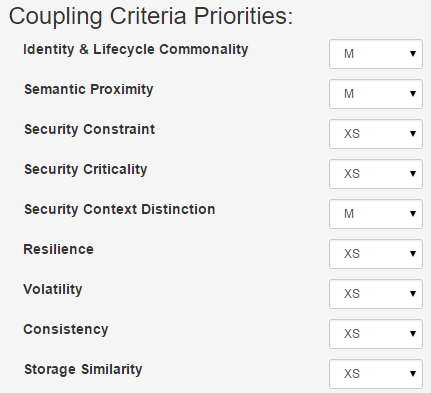
\includegraphics[scale=0.5]{images/priorities.png}
			\caption{Screenshot of default priorities in the Service Cutter}
			\label{fig:priorities}
		\end{center}
	\end{figure}
\end{minipage}

\subsection{Scoring Logic}

This section documents how each coupling criterion calculates its criterion score from $-10$ to $10$. 

Figure \ref{fig:scorer} shows the CriterionScorer interface used to calculate criterion scores. 

%TODO update
\begin{figure}[H]
	\begin{center}
		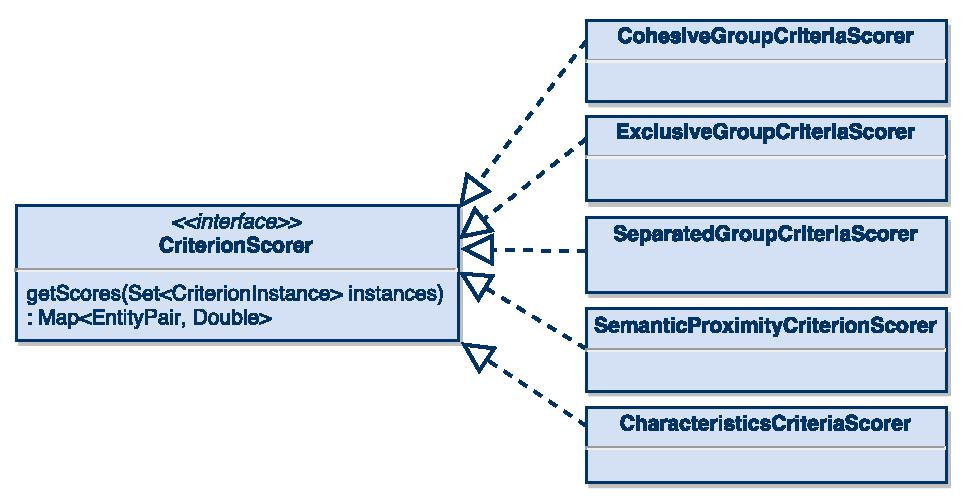
\includegraphics[scale=0.7]{diagrams/scorer.pdf}
		\caption{CriterionScorer Interface and its implementations}
		\label{fig:scorer}
	\end{center}
\end{figure}

%ZIO: how does this match implementation? previous section content?

%TODO implement other scorer and update
Currently there are four CriterionScorer implementations for different coupling criteria. Not all criteria have a suitable implementation yet, as we prioritized the criteria during the project as there was not enough time to implement the scoring for all criteria. Table \ref{tab:scorer} outlines which implementation is used for which coupling criterion.

\begin{table}[H]
	\centering
	\caption{Coupling Criteria and their scorer implementation}
	\label{tab:scorer}
	\begin{tabular}{|p{170pt}|p{200pt}|}
		\hline	
		\textbf{Coupling Criteria} & \textbf{Scorer Implementation}  \\
		\hline
		Responsibility \newline Consistency Constraint \newline Identity \& Lifecycle Commonality  & CohesiveGroupCriteriaScorer \\
		\hline
		Predefined Service Constraint  & ExclusiveGroupCriteriaScorer \\ 
		\hline
		Security Constraint & SeparationCriteriaScorer \\
		\hline
		Semantic Proximity & SemanticProximityCriterionScorer \\
		\hline
		Change Similarty \newline Consistency \newline Resilience \newline Volatility \newline Storage Similarty \newline Security Criticality & CharacteristicsCriteriaScorer  \\
		\hline
		Mutability \newline Network Traffic Suitability \newline Latency \newline Security Contextuality & No Implementation  \\
		\hline
	\end{tabular}
\end{table}

%ZIO: too early to feature implementation?

%ZIO: why this grouping? how / why different from figure in mgmt summary? (catalog overview)

%ZIO: utter jump from high level (CC) to low level implementation

%ZIO: add some table and domain model to bridge gap + allow user / reader to follow. CC->SC

\subsubsection{CohesiveGroupCriteriaScorer}

A CohesiveGroupCriteriaScorer is used for the criteria \textit{Consistency Constraint}, \textit{Identity \& Lifecycle Commonality} and \textit{Responsibiltiy}. These criteria define one or more groups of nanoentities that for some reason should be kept together in one service.

The scorer sets the maximum score of $10$ for every relation between nanoentities inside a group. 

\subsubsection{ExclusiveGroupCriteriaScorer}

A ExclusiveGroupCriteriaScorer is used for the \textit{Predefined Service Constraint} criterion. The scorer implements the same logic as a CohesiveGroupCriteriaScorer, but additionally sets a penalty of $-10$ from a nanoentity inside a group to all other nanoentities which do not share the same group.

\subsubsection{SeparationCriteriaScorer}

A SeparationCriteriaScorer is used for the criterion \textit{Security Constraint}. The criterion defines two or more groups of nanoentities which should clearly be separated into different services for security reasons. 

The implementation sets a negative score of $-10$ from each nanoentity to all other nanoentities defined in other groups than the own one. 

\subsubsection{SemanticProximityCriterionScorer}

%TODO: name for UML diagram? 
The SemanticProximityCriterionScorer is a more complex scoring implementation. It considers use cases and aggregations within a UML diagram. To calculate the score, the scorer uses an intermediate score summing up occurrences of the following conditions for the nanoentities $A$ and $B$:

\begin{description}
	\item [READ\_ACCESS] $A$ and $B$ are both read in the same use case.
	\item [WRITE\_ACCESS] $A$ and $B$ are both written in the same use case.
	\item [MIXED\_ACCESS] One of $A$ or $B$ is read and the other one written in the same use case.
	\item [AGGREGATED\_ENTITY] $A$ belongs to an entity which has an aggregation to B's entity in UML diagram. 
\end{description}

For each occurrence a number is added to the intermediate score of the $AB$ relation. Currently the following numbers are implemented:

SCORE\_WRITE\_ACCESS: 10 \newline
SCORE\_READ\_ACCESS: 3  \newline
SCORE\_MIXED\_ACCESS: 3 \newline 
SCORE\_AGGREGATION: 1 \newline 

These values are only used for the intermediate score and are not to be confound with the criterion score of $-10$ to $10$. More important than the actual numbers are the relative differences to each other which define the importance of the occurrences. Our defaults listed above put a strong emphasis on mutual write access. 

To reduce the intermediate score to the criterion score, the following rules are applied:

\begin{itemize}
	\item The top 10\% of all relations with the highest intermediate score receive a criterion score of 10.
	\item The lowest intermediate score of the top 10\% defines the reference intermediate score. The other 90\% are calculated relatively to that reference and receive a criterion score between 0 and 10.
\end{itemize}

The calculation for the lower 90\% works as following:

%TODO Michi: verstehe ich nicht!

\begin{equation}
\frac{referenceIntermediateScore}{x} = 10
\end{equation}
\begin{equation}
x = \frac{referenceIntermediateScore}{10}
\end{equation}
\begin{equation}
criterionScore_{AB} = \frac{intermediateScore_{AB}}{X}
\end{equation}

Both the numbers counted for access or aggregation occurrences and the reduction to the criterion score have been experimentally evaluated. The algorithm documented here has proven to produce reasonable results for the example systems tested but might require further investigations for other systems. 

\subsubsection{CharacteristicsCriteriaScorer}
%TODO styles?

Each coupling criterion of type compatibility defines multiple characteristics. The idea of these criteria is to create services with as homogeneous nanoentities as possible. The scorer therefore sets negative scores for a relation between two nanoentities having different characteristics. 

As an example, the criterion \textit{Change Similarity} describes how often change requests need to be implemented that affect a nanoentity. A nanoentity can have the characteristic \textit{often, normal} or \textit{rarely}. Each characteristic has a number between $0$ and $10$ assigned:

Often: $10$ \newline
Normal: $4$ \textit{(default)} \newline
Rarely: $0$ \newline

Two nanoentities with different characteristics receive a negative score with the difference between the numbers. As an example, a nanoentity $A$ with characteristic \textit{often} and a nanoentity $B$ with characteristic \textit{normal} receive a criterion score of $-6$. 

It is important that the highest and lowest number have a difference of $10$ to fully use the range a criterion has to rate a relation. \newline In this case there is an intermediate value of $4$ for the \textit{normal} characteristic. In our experience the often changing nanoentities are the most interesting and have the highest impact on service decomposition. With using the number $4$ instead of $5$ for \textit{normal} we put an emphasis on \textit{often} as the differences to this characteristics become bigger. 

To improve usability we introduced default values so that a user does not need to define characteristics of all criteria for all nanoentities. 

Table \ref{tab:characteristics} outlines characteristics of all criteria with their values and defaults. Both, the numbers and defaults are configurable for advanced users to better suit a systems requirements. 

%ZIO: sorry, i'm lost (in details)...

\begin{table}[H]
	\centering
	\caption{Criteria characteristics with values and defaults}
	\label{tab:characteristics}
	\begin{tabular}{|p{100pt}|p{150pt}|}
		\hline	
		\textbf{Criterion} & \textbf{Characteristics} \\
		\hline
		Change Similarity & Often 10 \newline Normal 4 \textit{(default)} \newline Rarely 0 \\
		\hline
		Consistency & High 10 \textit{(default)} \newline Eventually 4 \newline Weak 0 \\
		\hline
		Resilience & Critical 10 \newline Normal 4 \textit{(default)} \newline Low 0 \\
		\hline
		Volatility & Often 10 \newline Regularly 5 \textit{(default)} \newline Rarely 0 \\
		\hline
		Storage Similarity & Huge 10 \newline Normal 3 \textit{(default)} \newline Tiny 0 \\
		\hline
		Security Criticality & Critical 10 \newline Internal 3 \textit{(default)} \newline Public 0 \\
		\hline
	\end{tabular}
\end{table}


\section{Prototype} 

This section introduces the prototypical implementation of the Service Cutter to verify the feasibility of the decomposition approach presented in the previous section.

\subsection{Design}

The design of the Service Cutter was intentionally not evaluated in detail. We therefore followed the recommendation of our industry partner and used Spring Boot\cite{springboot} and JHipster\cite{jhipster} as the underlying frameworks.

The main reasons were:

\begin{itemize}
\item Our industry partner uses them successfully.
\item Spring Boot is considered the way to go for Spring based applications nowadays.
\item JHipster is based on established technologies that are partially already familiar to us. Furthermore it provides a code generator and samples. This can noticeable speed up development especially in the prototyping area.
\item We were able to implement a technological proof of concept in a few days and did not face major obstacles.
\end{itemize}

For the reasons listed above, we implemented the web application component using JHipster and the Engine using Spring Boot combined with a web service library. Section \ref{subsec:technology} discusses the utilized technologies in more detail.

\subsection{Technology}
\label{subsec:technology}


\begin{minipage}[t]{0.5\textwidth}
\setlength{\parskip}{5pt plus 0.1pt}
	The Service Cutter is implemented as a three tier application.
	
	The first tier is the web \textit{browser} of the user. The single-page application is based on AngularJS\cite{angularjs} and uses a template based on Bootstrap\cite{bootstrap}. A REST API provides access to the Editor tier.
	
	The \textit{Editor} component is a web application based on the JHipster\cite{jhipster} framework. It provides the use the possibility to import this domain information using a JSON upload and feeds this information into the Engine. All security and user interface aspects are handled in this layer.
	
	The \textit{Engine} is the isolated component that holds all the code to calculate candidate service cuts. It is also based on Spring technologies and provides a REST web service. The Engine does not provide any security measures and it is therefore necessary to restrict access to the Engine. We recommend to achieve this using a Docker\cite{docker} internal network as described in Section \ref{subsec:infrastructure}.
	
	%TODO db/orm? -> spring data supports hibernate
	
\end{minipage}
\begin{minipage}[t]{0.5\textwidth}
	\begin{figure}[H]
		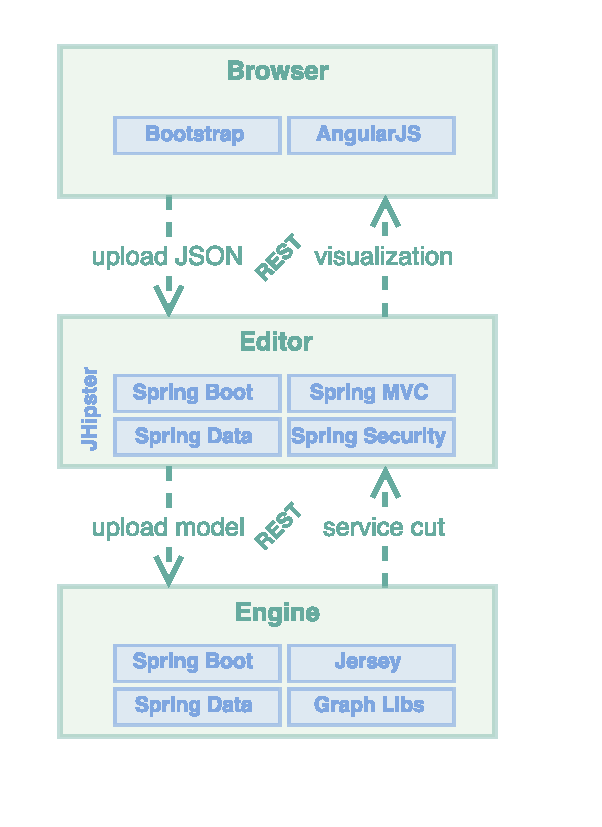
\includegraphics[scale=1]{diagrams/Technologies.pdf}
		\caption{Technology overview}
		\label{fig:technologies}
	\end{figure}
\end{minipage}


\subsection{Infrastructure}
\label{subsec:infrastructure}

Technically the Service Cutter can be operated on a single server providing a relational database and a Tomcat web server. However we developed a more sophisticated infrastructure aligned with modern standards which is presented as follows.

\begin{itemize}
\item Every components runs in an isolated Docker\cite{docker} container.
\item Docker Compose\cite{dockercompose} is used to link the Docker containers (hostnames, ports).
\item The Engine and the Editor operate in an embedded Tomcat server as provided by Sprint Boot web.
\item The Engine and the Editor both require a relational database. As Hibernate\cite{hibernate} and Liquibase\cite{liquibase} are used, all database related code is vendor agnostic. However we only tested the Service Cutter on Postgres 9.4\cite{postgres}.
\end{itemize}

Docker provides a layer of abstraction between the application and the underlying operating system. It uses resource isolation features of the Linux kernel to avoid the overhead of starting and maintaining full virtual machines. We implemented our deployment using Docker as it provides us with the ability to install the application components in isolated containers on a single machine with only a few command line statements.

The Docker Compose definition is attached in Appendix \ref{appendix:dockerCompose}.


\subsection{Graph Analyzing}

%TODO add text

\begin{figure}[H]
	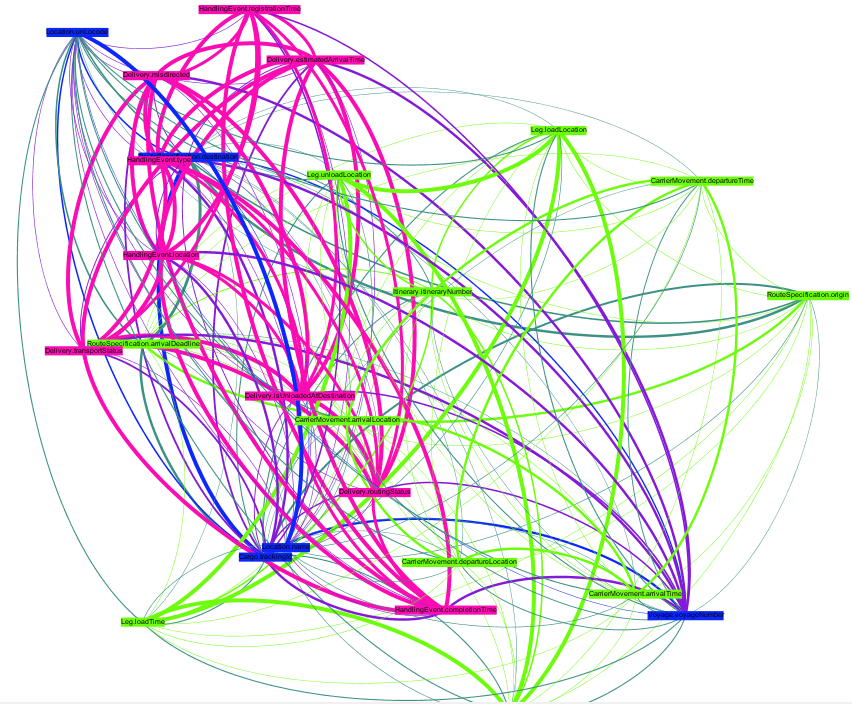
\includegraphics[scale=0.7]{images/ddd_semantic_proximity_debug.png}
	\caption{DDD Sample Graph Visualization with Gephi Platform}
	\label{fig:dddSampleGraph}
\end{figure}

\begin{figure}[H]
	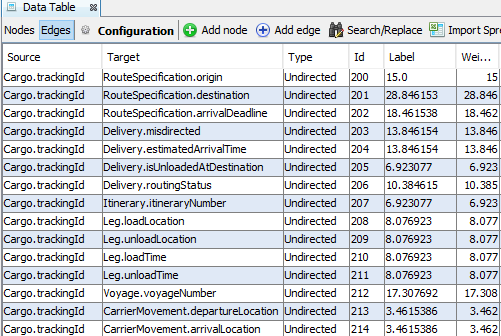
\includegraphics[scale=0.8]{images/ddd_semantic_proximity_debug_data.png}
	\caption{DDD Sample Graph Data Visualization with Gephi Platform}
	\label{fig:dddSampleData}
\end{figure}


\subsection{Information Security}

The web application is secured using an authentication and authorization implementation. Any other internal components such as the database or web services are hidden behind the servers firewall and therefore do not need any special security measures.

The uploaded data models are initially shared amongst all registered users.

\subsection{User Interface}

The base layout is responsive and adapts to smaller screens such as smartphones. However the tool is mostly used on devices such as laptops and the controls are therefore optimized for use on screens that are at least 15 inches wide and used with a mouse and a keyboard.


\bigskip
After covering the important design and implementation aspects, the next chapter explains how an architect can work with the Service Cutter.
